\chapter{\IfLanguageName{dutch}{Stand van zaken}{State of the art}}%
\label{ch:stand-van-zaken}

% Tip: Begin elk hoofdstuk met een paragraaf inleiding die beschrijft hoe
% dit hoofdstuk past binnen het geheel van de bachelorproef. Geef in het
% bijzonder aan wat de link is met het vorige en volgende hoofdstuk.

% Pas na deze inleidende paragraaf komt de eerste sectiehoofding.

Krachttraining omvat intensieve oefeningen die het lichaam blootstellen aan hoge fysieke eisen en zware belastingen. 
Dit kan leiden tot blessures ten gevolge van overbelasting, verkeerde liftingtechnieken en onvoldoende rust. 
De meeste blessures treden op tijdens de uitvoering van de squat, bench press en deadlift. 

\medskip

Volgens \textcite{BengtssonEtAl2018} is het essentieel om de liftingtechniek te analyseren en te optimaliseren, evenals de trainingsbelasting en rusttijden, om het risico op blessures te verminderen.
In dit opzicht biedt Artificiële Intelligentie, en meer specifiek Computer Vision en Pose Estimation, veelbelovende mogelijkheden.
Deze technologieën maken het mogelijk om menselijke bewegingen automatisch te analyseren en fouten in techniek vroegtijdig te detecteren. 
Door gebruik te maken van AI-gestuurde feedbacksystemen kunnen sporters hun houding en bewegingen optimaliseren, wat het risico op blessures aanzienlijk verkleint. 
Hiermee vormt AI een innovatieve aanvulling op traditionele trainingsmethoden en opent het de deur naar gepersonaliseerde, data-gedreven krachttrainingsbegeleiding, zelfs buiten de sportschoolomgeving.

\section{Basisoefeningen in powerlifting}
\label{sec:basisoefeningen-in-powerlifting}
De belangrijkste powerlifting-oefeningen zijn de squat, bench press en deadlift, die samen de basis van de sport vormen en de kwalificatie van de atleet bepalen \autocite{TymchikEtAl2021}. 
Elke oefening heeft specifieke kenmerken en technische vereisten.

\subsection{Squat}
\label{subsec:squat}
Bij de \textbf{conventionele squat} staat de atleet met een halter op de schouders, zakt door de benen tot een bepaalde diepte en komt weer omhoog. 
Het doel is om het maximale gewicht te squatten, waarbij niet alleen de beenspieren, maar ook andere spieren, met name de rugspieren, betrokken zijn.

\paragraph{Correcte uitvoering van de squat:}
Een correct uitgevoerde squat begint met je voeten op schouderbreedte of iets breder (circa 1,2-1,5 keer je schouderbreedte), met je tenen recht naar voren of maximaal 7-10 graden naar buiten gedraaid \autocite{LorenzettiEtAl2018}. 
De ganse voet moet contact houden met de grond, vooral de hielen moeten stevig blijven staan \autocite{CzaprowskiEtAl2012}. 
Tijdens het zakken moeten de knieën in lijn blijven met de tenen en mogen ze ongeveer 5-10 cm voorbij de tenen komen, in een hoek van zo'n 45 graden ten opzichte van de romp \autocite{LorenzettiEtAl2018}.

\medskip

Vervolgens dient men gecontroleerd naar beneden te zakken tot de knieën minstens een hoek van 90 graden maken (halve squat), of nog dieper tot de dijen parallel aan de grond zijn (115-125 graden knieflexie) voor meer betrokkenheid van de bilspieren \autocite{ComfortEtAl2018}. 
De rug recht moet recht gehouden worden met een natuurlijke licht gebogen vorm in de lumbale lordose (onderrug).
Een thoracale kyfose (bolle bovenrug) dient absoluut vermeden te worden.
De romp helt vanzelf iets naar voor, onder een hoek van ongeveer 45 graden bij een volledige squat \autocite{CzaprowskiEtAl2012}.

De beweging begint steeds door de heupen naar achteren te duwen en vervolgens wordt een gecontroleerd tempo aangehouden - ongeveer 2-3 seconden voor het zakken en 1-2 seconden voor het omhoog komen \autocite{CzaprowskiEtAl2012}.

\begin{figure}[h]
  \centering
  % Eerste afbeelding
  \begin{minipage}[t]{0.32\textwidth}
    \centering
    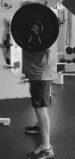
\includegraphics[height=6cm,width=\textwidth,keepaspectratio]{squat_start_pos.png}
    \caption[Startpositie squat]{\label{fig:squat_startpositie} Startpositie \autocite{RonaiEtAl2023}}
  \end{minipage}
  \hfill
  % Tweede afbeelding
  \begin{minipage}[t]{0.32\textwidth}
    \centering
    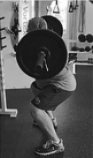
\includegraphics[height=6cm,width=\textwidth,keepaspectratio]{squat_middle_pos.png}
    \caption[Middenpositie squat]{\label{fig:squat_middenpositie} Middenpositie \autocite{RonaiEtAl2023}}
  \end{minipage}
  \hfill
  % Derde afbeelding
  \begin{minipage}[t]{0.32\textwidth}
    \centering
    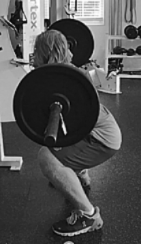
\includegraphics[height=6cm,width=\textwidth,keepaspectratio]{squat_bottom_pos.png}
    \caption[Onderste positie squat]{\label{fig:squat_onderpositie} Laagste positie \autocite{RonaiEtAl2023}}
  \end{minipage}
\end{figure}


\subsection{Bench Press}
\label{subsec:bench-press}
Bij de \textbf{bench press} ligt de atleet op een bank, laat een halter zakken tot de borst en drukt deze vervolgens weer omhoog. 
Het doel is om het maximale gewicht te bankdrukken, waarbij technische aspecten zoals de positie van de voeten, schouders, gripbreedte en het neerlaten van de halter op de borst cruciaal zijn.

\paragraph{Correcte uitvoering van de bench press:}
De correcte houding bij het uitvoeren van de bench press begint met een stabiele lichaamspositie op de bank. 
Men ligt op de rug met het hoofd, de schouders en heupen volledig in contact met de bank. 
De voeten staan plat op de vloer op ongeveer schouderbreedte uit elkaar, waarbij een natuurlijke kromming in de onderrug wordt aangehouden zonder overdreven holle rug. 
Voor de standaardtechniek zijn vijf contactpunten essentieel: het hoofd, de schouderbladen, de bovenrug en de billen houden contant met de bank, terwijl beide voeten stevig op de grond staan \autocite{KrolEtAl2010}.

\medskip

Men neemt een bovenhandse greep waarbij de handen iets wijder dan schouderbreedte staan, ongeveer 1,5 keer de afstand tussen de schouderpunten. 
Een te brede greep (meer dan 2,5 keer de schouderbreedte) belast het AC-gewricht (acromioclaviculair gewricht, verbinding tussen sleutelbeen en schouderdak) onnodig, terwijl een smallere greep deze belasting juist kan verminderen \autocite{Ronai2018}. 
De stang dient gelijkmatig ten opzichte van het midden, vastgepakt te worden \autocite{KrolEtAl2010}.

\medskip

Voordat men begint, worden de schouderbladen actief naar elkaar toe en omlaag getrokken om een stevige basis te creëren en instabiliteit in het schoudergewricht te voorkomen \autocite{NoteboomEtAl2024}. 
Men start met licht gebogen ellebogen en houd de polsen stijf, recht boven de ellebogen uitgelijnd. 
Men laat de stang gecontroleerd zakken naar borsthoogte (ongeveer ter hoogte van de tepels) in 1-3 seconden, waarbij elk stuiteren wordt vermeden. 
Men houdt de bovenarmen in een hoek van ongeveer 45 graden ten opzichte van het torso om overmatige belasting van de schouders te voorkomen \autocite{Ronai2018}. 
Vervolgens wordt de stang krachtig omhoog geduwt in 1-2 seconden tot de ellebogen volledig gestrekt zijn, waarbij de stang zich boven de ogen bevindt en een lichte boog naar achteren beschrijft.

\begin{figure}[h]
  \centering
  % Eerste afbeelding
  \begin{minipage}[t]{0.32\textwidth}
    \centering
    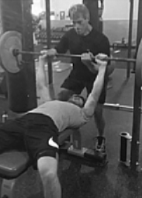
\includegraphics[height=6cm,width=\textwidth,keepaspectratio]{bench_starting_pos.png}
    \caption[Startpositie bench press]{\label{fig:bench_startpositie} Startpositie \autocite{Ronai2018}}
  \end{minipage}
  \hfill
  % Tweede afbeelding
  \begin{minipage}[t]{0.32\textwidth}
    \centering
    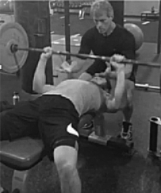
\includegraphics[height=6cm,width=\textwidth,keepaspectratio]{bench_middle_pos.png}
    \caption[Middenste positie bench press]{\label{fig:bench_middenpositie} Middenpositie \autocite{Ronai2018}}
  \end{minipage}
  \hfill
  % Derde afbeelding
  \begin{minipage}[t]{0.32\textwidth}
    \centering
    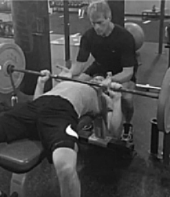
\includegraphics[height=6cm,width=\textwidth,keepaspectratio]{bench_bottom_pos.png}
    \caption[Onderste positie bench press]{\label{fig:bench_onderpositie} Laagste positie \autocite{Ronai2018}}
  \end{minipage}
\end{figure}

\subsection{Deadlift}
\label{subsec:deadlift}
De \textbf{conventionele deadlift} omvat het tillen van een halter van de grond tot een rechtopstaande positie met gestrekte rug en benen. 
Deze oefening wordt gezien als een indicator van absolute kracht in de rug en benen.

\paragraph{Correcte uitvoering van de deadlift:}
Een correct uitgevoerde deadlift begint met de voeten op heup- tot schouderbreedte, licht naar buiten gedraaid (ongeveer 10-15 graden). 
Vervolgens buigt men door de knieën en heupen (knieën ongeveer 20-30 graden gebogen) om de stang vast te pakken met een greep die net iets breder is dan schouderbreedte. 
Het bovenlichaam vormt hierbij een hoek van 30-45 graden met de vloer. 
Men zorgt ervoor dat de schouders recht boven of net voor de stang zijn, de borst naar voren geduwd is en de rug recht blijft met een natuurlijke licht gebogen vorm in de lumbale lordose (onderrug) \autocite{BirdEtAl2010}. 
De stang moet tegen de scheenbenen aan liggen, ongeveer ter hoogte van het midden van de voet \autocite{Ronai2020}.

\medskip

Bij het optillen strekt men de heupen en knieën gelijktijdig, waarbij men de stang dicht langs het lichaam houdt. 
Een belangrijk aandachtspunt is wanneer de bovenbenen een hoek van ongeveer 60 graden bereiken - dit is vaak het lastigste punt in de beweging. 
Men eindigt rechtop met volledig gestrekte heupen en knieën (maar niet overstrekt), waarbij het lichaam een rechte verticale lijn vormt \autocite{Ronai2020}.

\medskip

Bij het opnieuw laten zakken van de halterstang scharniert men de heupen naar achteren (ongeveer 15 graden) voordat men de knieën buigt.
De stang wordt opnieuw dicht langs het lichaam gehouden en de recht rugpositie blijft behouden tijdens deze neerwaartse beweging.
Het gewicht wordt verdeelt over de ganse voet, met iets meer nadruk op de hielen en de middenvoet \autocite{Ronai2020}

\begin{figure}[h]
  \centering
  % Eerste afbeelding
  \begin{minipage}[t]{0.32\textwidth}
    \centering
    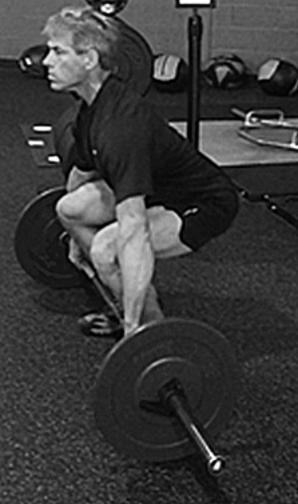
\includegraphics[height=6cm,width=\textwidth,keepaspectratio]{deadlift_bottom_pos.png}
    \caption[Startpositie deadlift]{\label{fig:deadlift_startpositie} Startpositie \autocite{Ronai2020}}
  \end{minipage}
  \hfill
  % Tweede afbeelding
  \begin{minipage}[t]{0.32\textwidth}
    \centering
    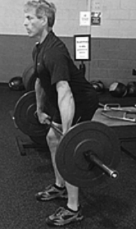
\includegraphics[height=6cm,width=\textwidth,keepaspectratio]{deadlift_middle_pos.png}
    \caption[Middenste positie deadlift]{\label{fig:deadlift_middenpositie} Middenpositie \autocite{Ronai2020}}
  \end{minipage}
  \hfill
  % Derde afbeelding
  \begin{minipage}[t]{0.32\textwidth}
    \centering
    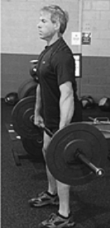
\includegraphics[height=6cm,width=\textwidth,keepaspectratio]{deadlift_upper_pos.png}
    \caption[Hoogste positie deadlift]{\label{fig:deadlift_bovenpositie} Hoogste positie \autocite{Ronai2020}}
  \end{minipage}
\end{figure}

\section{Gevaren van een verkeerde liftingtechniek}
\label{sec:gevaren-verkeerde-liftingtechniek}
De liftingtechniek is een cruciale factor bij powerliften en heeft een aanzienlijke invloed op het risico op blessures. 
Naast het managen van trainingsbelasting, is het optimaliseren van de liftingtechniek het belangrijkste preventieve middel tegen blessures \autocite{StrömbäckEtAl2018}. 
Een suboptimale techniek is in verband gebracht met blessures, hoewel er onder onderzoekers, coaches en atleten discussie bestaat over wat een correcte techniek precies inhoudt. 
Hieronder worden de belangrijkste aspecten van de liftingtechniek bij de squat, bench press en deadlift besproken, evenals enkele algemene overwegingen.

\subsection{Risicofactoren bij de squat}
\label{subsec:risicofactoren-squat}
Bij de \textbf{squat} kunnen variaties in de techniek de krachten op de gewrichten beïnvloeden. 
\textcite{BengtssonEtAl2018} geven aan dat factoren zoals squatdiepte, standbreedte, bewegingssnelheid, barbell-positie en blikrichting spelen een rol bij het blessurerisico. 
Een grotere knieflexie verhoogt bijvoorbeeld de compressie- en schuifkrachten, terwijl knieflexie, heup adductie (beweging naar de middellijn toe) en interne rotatie van de femur (dijbeen) punten van aandacht zijn.
Een te brede stand kan de compressiekrachten op de knie verhogen, terwijl een smalle stand de anterieure schuifkrachten kan vergroten. 
Een hogere liftsnelheid of een stuiterende beweging onderaan de squat verhoogt de schuifkrachten op de knie, terwijl een snelle en ongecontroleerde afdaling de spanning op de kruisbanden en collaterale ligamenten (zijdelingse kniebanden) kan vergroten. 
Daarnaast is een grotere voorwaartse leun geassocieerd met verhoogde lumbale schuifkrachten (schuifkrachten in de onderrug), en een hoge barbellpositie verplaatst de belasting van de heupen naar de knieën. 
Een neerwaartse blik kan de heupflexie en rompflexie vergroten.

\begin{figure}[h]
  \centering
  \begin{minipage}{0.45\textwidth}
      \centering
      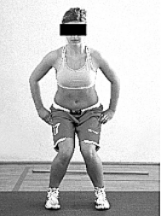
\includegraphics[width=\linewidth]{squat_bad_knees.png}
      \caption[Squat met incorrecte positie van de knieën]{\label{fig:squat_incorrect}Squat met incorrecte positie van de knieën \autocite{CzaprowskiEtAl2012}}
  \end{minipage}
  \hfill % Voegt wat ruimte toe tussen de afbeeldingen
  \begin{minipage}{0.45\textwidth}
      \centering
      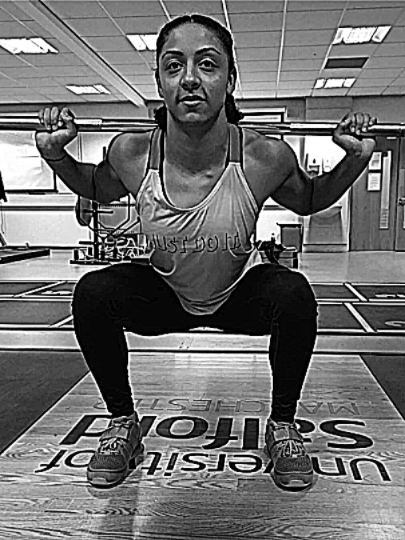
\includegraphics[width=\linewidth]{squat_good_knees.png}
      \caption[Squat met correcte positie van de knieën]{\label{fig:squat_correct}Squat met correcte positie van de knieën\autocite{ComfortEtAl2018}}
  \end{minipage}
\end{figure}

\subsection{Risicofactoren bij de bench press}
\label{subsec:risicofactoren-bench-press}
Bij de \textbf{bench press} wordt de oefening vaak gezien als een risicofactor voor schouderblessures. 
Hier halen \textcite{BengtssonEtAl2018} aan dat factoren zoals gripbreedte, schouderpositie en het al dan niet trekken van een boog in de rug kunnen het blessurerisico beïnvloeden. 
Een brede grip kan de schouder in een nadelige positie plaatsen, wat belasting geeft aan het acromioclaviculaire gewricht (verbinding tussen sleutelbeen en schouderdak), de glenohumerale ligamenten (banden rond het schoudergewricht) en de pectoralis major spier (grote borstspier). 
Een wijdere grip verhoogt ook de schoudertorsie, wat de eisen aan de rotator cuff (groep schouderkapselspieren) en bicepspees complex vergroot. 
Het verliezen van controle over de barbell kan leiden tot fracturen en schouderdislocaties (ontwrichtingen).

\begin{figure}[h]
  \centering
  \begin{minipage}{0.45\textwidth}
      \centering
      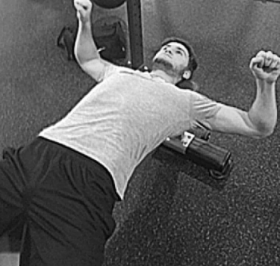
\includegraphics[width=\linewidth]{bench_bad_elbows.png}
      \caption[Bench press met incorrecte positie van de ellebogen]{\label{fig:bench_incorrect}Bench press met incorrecte positie van de ellebogen \autocite{Ronai2018}}
  \end{minipage}
  \hfill % Voegt wat ruimte toe tussen de afbeeldingen
  \begin{minipage}{0.45\textwidth}
      \centering
      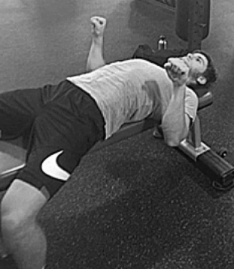
\includegraphics[width=\linewidth]{bench_good_elbows.png}
      \caption[Bench press met correcte positie van de ellebogen]{\label{fig:bench_correct}Bench press met correcte positie van de ellebogen \autocite{Ronai2018}}
  \end{minipage}
\end{figure}    

\subsection{Risicofactoren bij de deadlift}
\label{subsec:risicofactoren-deadlift}
Bij de \textbf{deadlift} wordt een rechte torso met behoud van lumbale lordose (natuurlijke kromming van de onderrug) verondersteld het blessurerisico te verminderen. 
Het dicht bij het lichaam houden van de barbell is belangrijk, omdat dit de heup- en spinale momentarmen (hefboomwerking op wervelkolom) verkleint en zo de prestaties verbetert en het blessurerisico vermindert. 
Het is ook essentieel om de knieën niet voortijdig of overmatig te strekken om een 'stiff-leg' deadlift te voorkomen \autocite{BengtssonEtAl2018}.

\begin{figure}[h]
  \centering
  \begin{minipage}{0.45\textwidth}
      \centering
      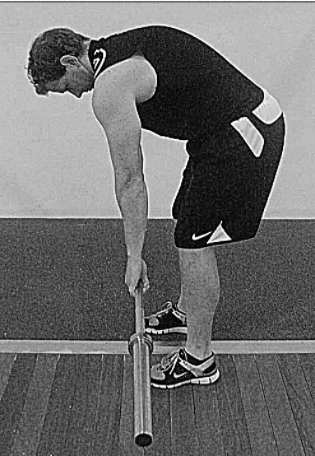
\includegraphics[width=\linewidth]{deadlift_bad_posture.png}
      \caption[Deadlift met incorrecte houding]{\label{fig:deadlift_incorrect}Deadlift met incorrecte houding \autocite{BirdEtAl2010}}
  \end{minipage}
  \hfill % Voegt wat ruimte toe tussen de afbeeldingen
  \begin{minipage}{0.45\textwidth}
      \centering
      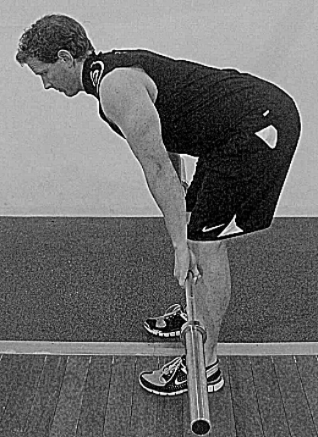
\includegraphics[width=\linewidth]{deadlift_good_posture.png}
      \caption[Deadlift met correcte houding]{\label{fig:deadlift_correct}Deadlift met correcte houding \autocite{BirdEtAl2010}}
  \end{minipage}
\end{figure}   

\subsection{Algemene overwegingen}
Naast de specifieke technieken per oefening zijn er algemene overwegingen. De combinatie van zware lasten en een onjuiste techniek verhoogt het blessurerisico aanzienlijk. 
Vermoeidheid kan de techniek negatief beïnvloeden, en het is belangrijk om te analyseren of een bewegingspatroon een adaptieve of maladaptieve reactie op pijn is.

Het optimaliseren of veranderen van het bewegingspatroon kan pijn verminderen, en als dit het geval is, moeten de onderliggende bewegingssysteemverstoringen die het niet-optimale patroon veroorzaken, worden hersteld. 
Dit benadrukt het belang van technische precisie en aanpassing aan individuele behoeften om blessures te voorkomen en prestaties te optimaliseren \autocite{TymchikEtAl2021}.

\medskip

Door deze technische richtlijnen nauwkeurig toe te passen bij alle powerlifting-oefeningen, kunnen atleten niet alleen hun krachtontwikkeling maximaliseren, maar ook het risico op blessures aanzienlijk verkleinen.

\section{\IfLanguageName{dutch}{Artificiële Intelligentie}{Artificial Intelligence}}%
\label{sec:artificiële-intelligentie}

Artificiële Intelligentie (AI) is een dynamisch en snel evoluerend vakgebied dat zich richt op het ontwikkelen van systemen die taken kunnen uitvoeren die normaal gesproken menselijke intelligentie vereisen, zoals leren, probleemoplossing en besluitvorming \autocite{SharifaniEtAl2023}.
Het doel is om machines te ontwikkelen die autonoom kunnen functioneren in complexe en dynamische omgevingen \autocite{Kouassi2023}.

\medskip

AI als vakgebied is al meer dan 65 jaar in ontwikkeling en heeft zich inmiddels diep genesteld in ons dagelijks leven. Het speelt immers een curicale rol in sectoren zoals gezondheidszorg, transport, onderwijs en industrie, en wordt gezien als een belangrijke drijfveer voor sociaaleconomische veranderingen en technologische vooruitgang \autocite{JiangEtAl2022}.

\medskip

Binnen AI zijn Machine Learning (ML) en Deep Learning (DL) twee van de meest revolutionaire technologieën, die de afgelopen jaren aanzienlijke vooruitgang hebben geboekt \autocite{SharifaniEtAl2023}.

\begin{figure}
  \centering
  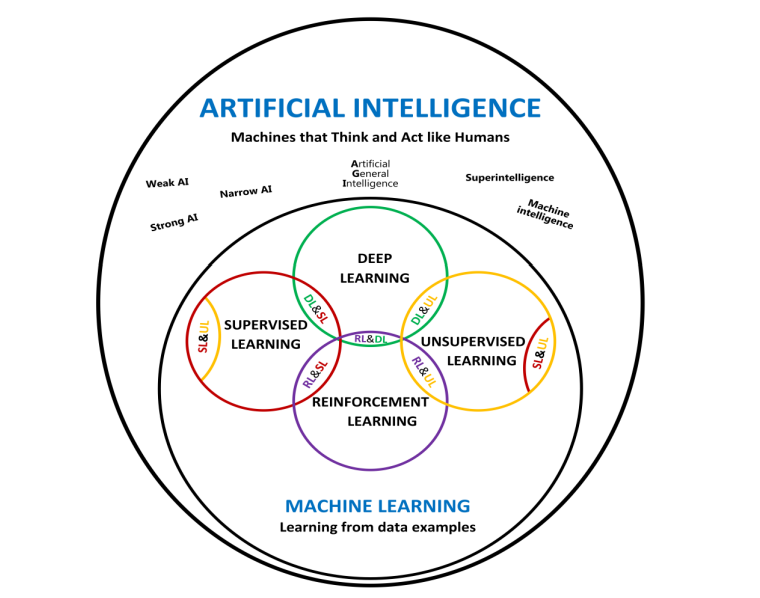
\includegraphics[width=0.8\textwidth]{ai.png}
  \caption[AI landschap]{\label{fig:ai}Het AI landschap met zijn verschillende technieken \autocite{Kouassi2023}}
\end{figure}

\subsection{\IfLanguageName{dutch}{Machine Learning}{Machine Learning}}%
\label{subsec:machine-learning}

ML is momenteel de meest dominante vorm van AI. Het is een methode voor data-analyse die het mogelijk maakt om analytische modellen automatisch te bouwen en te verbeteren. Het stelt computers in staat om te leren van ervaring, zonder expliciet te worden geprogrammeerd \autocite{SharifaniEtAl2023}.

\medskip

ML omvat de volgende technieken, die gecombineerd kunnen worden om nog krachtigere en veelzijdigere AI-systemen te ontwikkelen \autocite{Kouassi2023}. 

\begin{itemize}
  \item \textbf{Supervised Learning (SL)}: Hierbij wordt een model getraind met behulp van gelabelde gegevens, waarbij zowel de invoer als de gewensteuitvoer bekend zijn. Het model leert in feite door voorbeelden, vergelijkbaar met een leerling die oefent met vragen en de bijbehorende antwoorden. Het doel is om patronen te herkennen die vervolgens kunnen worden gebruikt om voorspellingen te maken voor nieuwe, onbekende gegevens. Voorbeelden van toepassingen zijn het herkennen van spam en het classificeren van afbeeldingen.
  \item \textbf{Unsupervised Learning (UL)}: Deze techniek werkt met ongelabelde data, waarbij het model zelf patronen of structuren moet ontdekken. Dit gebeurt vaak door clustering, waarbij vergelijkbare data automatisch worden gegroepeerd. Een voorbeeld is het segmenteren van klanten op basis van koopgedrag. UL is vooral nuttig wanneer er geen duidelijke labels beschikbaar zijn. 
  \item \textbf{Reinforcement Learning (RL)}: RL draait om een model dat leert door interactie met een omgeving. Het model probeert een strategie (beleid) te ontwikkelen die maximale beloningen oplevert. Dit wordt vaak gebruikt in scenario's zoals robotica, gaming en autonome voertuigen, waarbij het model leert door trial-and-error. 
\end{itemize}

\subsection{\IfLanguageName{dutch}{Deep Learning}{Deep Learning}}%
\label{subsec:deep-learning}

Dit is een geavanceerde vorm van ML die gebruikmaakt van gelaagde neurale netwerken, geïnspireerd op de structuur van het menselijk brein.
Het model verwerkt data iteratief, waarbij het parameters aanpast op basis van feedback.  
Het is vooral geschikt voor taken met grote hoeveelheden ongestructureerde data, zoals beeld- en spraakherkenning. 
In tegenstelling tot traditionele ML modellen kan DL automatisch hoogwaardige kenmerken uit data halen, waardoor het beter presteert bij ingewikkelde taken \autocite{SharifaniEtAl2023}.
De bekomen kenmerken kunnen vervolgens door het DL model zelf gebruikt worden of geïntegreerd worden in andere ML-modellen \autocite{JanieschEtAl2021}. 

Er zijn verschillende DL-architecturen, waarvan Convolutionele Neurale Netwerken (CNN's) en Recurrente Neurale Netwerken (RNN's) de meest bekende vormen.

\begin{itemize}
    \item \textbf{Convolutional Neural Networks (CNNs):} 
    CNNs zijn deep learning-modellen die vooral worden gebruikt voor taken met afbeeldingen, zoals beeldclassificatie, objectdetectie en semantische segmentatie. Ze bestaan uit convolutielagen die kenmerken (features) uit afbeeldingen halen met behulp van filters (kernels), poolinglagen die de afbeelding verkleinen en belangrijke informatie behouden, en volledig verbonden lagen die de kenmerken combineren voor taken zoals classificatie. Activatie-functies helpen het model om complexe patronen te leren. CNNs zijn ideaal voor visuele data vanwege hun vermogen om ruimtelijke patronen te herkennen \autocite{ZhaoEtAl2024}.

    \item \textbf{Recurrent Neural Networks (RNNs):} 
    RNNs zijn deep learning-modellen die geschikt zijn voor sequentiële data, zoals tijdreeksen, tekst en gebeurtenissen. Ze hebben interne feedback-lussen die informatie van eerdere stappen onthouden, waardoor ze tijdafhankelijke patronen kunnen modelleren. Elke stap in de reeks wordt verwerkt met informatie uit vorige stappen, wat RNNs ideaal maakt voor taken zoals tijdreeksvoorspelling, tekstgeneratie en machinevertaling. RNNs zijn krachtig vanwege hun geheugen en vermogen om sequentiële relaties te leren \autocite{JanieschEtAl2021}.
\end{itemize}

\begin{figure}
  \centering
  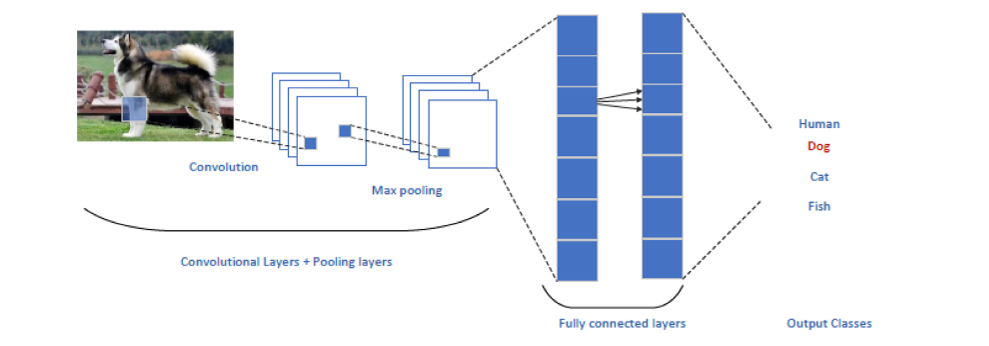
\includegraphics[width=0.8\textwidth]{cnn.png}
  \caption[CNN classificatie van een afbeelding]{\label{fig:cnn}CNN architectuur voor de classificatie van een afbeelding \autocite{ChaiEtAl2021}}
\end{figure}



Kortom, Deep Learning is een krachtige en veelzijdige technologie die een centrale rol speelt in de moderne AI-revolutie. 
Het is bijzonder effectief in het verwerken van grote en complexe datasets en heeft toepassingen in tal van domeinen. 
Echter, de ontwikkeling van DL-modellen brengt ook uitdagingen met zich mee, zoals het optimaliseren van modellen en het integreren van logisch redeneren. 
DL blijft een belangrijk onderzoeksgebied met een groot potentieel voor toekomstige innovaties \autocite{JiangEtAl2022}.

\subsection{\IfLanguageName{dutch}{Computer Vision}{Computer Vision}}%
\label{subsec:computer-vision}

Computer Vision (CV) is een snelgroeiend vakgebied binnen de beeldverwerking, waarbij CNN's, een belangrijk onderdeel van DL, een centrale rol spelen.  

\medskip

In de beginfase van CV werden DL-methoden beperkt door technische uitdagingen, zoals beperkt geheugen en rekenkracht. 
Hierdoor lag de focus aanvankelijk op traditionele ML-technieken. 
Met de verbetering van hardware (CPU/GPU) en de ontwikkeling van krachtige DL-modellen werd DL echter de dominante benadering in CV \autocite{ChaiEtAl2021}.

\medskip

CNN's hebben een revolutie teweeggebracht in taken zoals beeldclassificatie, objectdetectie en beeldreconstructie. 
Ze leren automatisch kenmerken uit ruwe data, waardoor ze complexe patronen kunnen herkennen en hogere niveau-representaties kunnen vormen. 
Dit maakt ze ideaal voor praktische toepassingen. 

\medskip

CV wordt breed ingezet in domeinen zoals autonoom rijden (object- en verkeersherkenning), virtual reality (immersieve ervaringen), en intelligente videobewaking (detectie van verdachte activiteiten). 
Ook wordt het gebruikt voor Human Activity Recognition (HAR), zoals het monitoren van ouderen of revalidatie, en voor taken zoals spraakherkenning en sentimentanalyse. 

\medskip

Een belangrijke uitdaging is dat CNN's veel rekenkracht en grote hoeveelheden gelabelde data vereisen, wat kostbaar en tijdrovend kan zijn. 
Toch blijft het veld zich snel ontwikkelen, met toekomstige richtingen zoals ensemble learning (combinatie van meerdere CNN's), aandachtsmechanismen (gericht op belangrijke informatie in beelden) \autocite{ZhaoEtAl2024}. 

\subsubsection{\IfLanguageName{dutch}{Pose Estimation}{Pose Estimation}}%
\label{subsubsec:pose-estimation}
 
Pose Estimation is een CV-techniek die menselijke poses schat door lichaamsdelen en gewrichtsposities te detecteren in afbeeldingen of video's. 
Het wordt gebruikt in toepassingen zoals games, animatie, medische analyse, AI-gestuurde persoonlijke trainers, human-computer interactie, bewegingsanalyse, augmented reality, virtual reality, posetracking, actieherkenning en surveillance systemen \autocite{SiddharthEtAl2021}.

\medskip

Pose estimation maakt gebruik van twee hoofdbenaderingen om de positie en oriëntatie van objecten (zoals mensen) in afbeeldingen of video's te schatten: \textbf{top-down} en \textbf{bottom-up} methoden. 
Beide methoden hebben hun eigen sterke en zwakke punten, afhankelijk van de toepassing.

\begin{itemize}
    \item \textbf{Top-down methoden:} 
    Deze benadering begint met het detecteren van een persoon in de afbeelding. 
    Vervolgens wordt een bounding box (een kader) rond de persoon getrokken, waarbinnen de pose wordt geschat. 
    Dit gebeurt door een 2D heatmap te genereren voor elk gewricht, zoals ellebogen of knieën. 
    Top-down methoden zijn zeer effectief voor het detecteren van één persoon en bieden nauwkeurige pose-schattingen binnen de bounding box. 
    Ze zijn echter minder geschikt voor situaties met meerdere personen, vooral wanneer er overlapping (occlusies) optreedt \autocite{LiuEtAl2022}.

    \item \textbf{Bottom-up methoden:} 
    In tegenstelling tot top-down methoden, detecteren bottom-up methoden eerst alle gewrichtspunten (keypoints) van alle personen in de afbeelding. 
    Vervolgens worden deze punten gecombineerd op basis van de structuur van het menselijk lichaam om de pose te schatten. 
    Deze aanpak is beter geschikt voor het detecteren van meerdere personen in één afbeelding en is minder gevoelig voor occlusies. 
    Bottom-up methoden zijn echter complexer om te implementeren vanwege de noodzaak om keypoints correct te combineren \autocite{BeomjunEtAl2022}.
\end{itemize}

Het doel van pose estimation is om de 3D-positie en oriëntatie van een object te bepalen op basis van zijn 2D-projectie in een afbeelding of video. 
Dit wordt bereikt door de 2D-locaties van keypoints (zoals gewrichten) te schatten en deze om te zetten naar een 3D-representatie \autocite{SulongEtAl2023}. 
Beide methoden, top-down en bottom-up, spelen een cruciale rol in computer vision-toepassingen, zoals sportanalyse, augmented reality en robotica.

\medskip

Convolutional Neural Networks (CNN's) spelen een centrale rol hierby, waarbij ze worden getraind om lichaamsdelen te classificeren en ruimtelijke modellen te combineren voor nauwkeurige resultaten. 
Andere geavanceerde technieken zijn Transformers (voor langeafstandsafhankelijkheden), Graph Convolutional Networks (voor correlaties tussen gewrichten) en Adversarial Learning (om robuustheid en nauwkeurigheid te verbeteren). 
Moderne methoden zoals DeepPose (gebruikt Deep Neural Networks), Adversarial PoseNet (combineert generatoren en discriminatoren voor nauwkeurige heatmaps) en OpenPose (real-time multi-person schatting met Part Affinity Fields) hebben het veld aanzienlijk vooruit geholpen \autocite{ZhaoEtAl2024}.

\medskip

Kortom, Human Pose Estimation (HPE) is een veelzijdige techniek met brede toepassingen, ondersteund door geavanceerde modellen en aandacht voor uitdagingen zoals occlusies en schaalvariaties. 
Door de inzet van deep learning-technieken en innovatieve benaderingen blijft het veld zich snel ontwikkelen, met als doel real-time, nauwkeurige en robuuste pose-schatting mogelijk te maken \autocite{DongEtAl2024}.


\paragraph{\IfLanguageName{dutch}{Uitdagingen van Pose Estimation op mobiele apparaten}{Challenges for Pose Estimation on Mobile Devices}}%
\label{par:uitdagingen-van-pose-estimation-op-mobiele-apparaten}

Desondanks Pose Estimation al enorme technologische vooruitgang geboekt heeft, zijn er nog steeds enkele uitdagingen om modellen te integreren in mobiele applicaties.

\begin{itemize}
    \item \textbf{Beperkte Rekenkracht}: 
    Mobiele apparaten hebben minder hardwarecapaciteit dan servers of computers, waardoor het gebruik van complexe en grote neurale netwerken moeilijk is. Pose estimation-algoritmen vereisen vaak veel rekenkracht, wat kan leiden tot trage prestaties en een hoog energieverbruik \autocite{LiuEtAl2022}.

    \item \textbf{Modelgrootte}: 
    Voor mobiele toepassingen moeten modellen compact zijn om efficiënt te kunnen draaien. Grote modellen zijn vaak niet geschikt vanwege beperkte opslag en geheugen op mobiele apparaten \autocite{HouEtAl2020}.

    \item \textbf{Real-time Prestaties}: 
    Pose estimation moet in real-time werken, vooral voor toepassingen zoals fitness-tracking of augmented reality. Vertragingen kunnen de gebruikerservaring negatief beïnvloeden \autocite{HouEtAl2020}.

    \item \textbf{Wisselende Omstandigheden}: 
    Mobiele apparaten worden in diverse omgevingen gebruikt, wat pose estimation uitdagend maakt. Factoren zoals camerarotaties, wisselende belichting, en occlusies (bijvoorbeeld wanneer lichaamsdelen elkaar overlappen) kunnen de nauwkeurigheid verminderen \autocite{SulongEtAl2023}.

    \item \textbf{Beperkte Trainingsdata}: 
    Het verzamelen van voldoende en gevarieerde trainingsdata is een uitdaging, wat de nauwkeurigheid van modellen kan beperken. Dit geldt vooral voor scenario’s met ongebruikelijke poses of achtergronden \autocite{PauloEtAl2024}.

    \item \textbf{Nauwkeurigheidsproblemen}: 
    Beeldvervorming, achtergrondruis of complexe objecten kunnen de nauwkeurigheid van pose estimation beïnvloeden. Dit is vooral problematisch bij objecten met ongebruikelijke vormen of structuren \autocite{SulongEtAl2023}.
\end{itemize}

Om de uitdagingen van pose estimation op mobiele apparaten het hoofd te bieden, zijn enkele praktische stappen nodig. Ten eerste is het belangrijk om een lichtgewicht model te kiezen dat minder rekenkracht vereist, maar toch goede prestaties levert. Dit maakt het mogelijk om real-time resultaten te behalen op mobiele hardware. Daarnaast moet het model getraind worden op diverse omstandigheden, zoals wisselende belichting, camerahoeken en occlusies, om de nauwkeurigheid in verschillende omgevingen te waarborgen.
\medskip
Ook is het nuttig om best practices voor training toe te passen, zoals het gebruik van synthetische data of transfer learning, vooral als er beperkte trainingsdata beschikbaar is. Dit helpt om het model robuuster en nauwkeuriger te maken. Ten slotte kan het gebruik van beschikbare tools en frameworks het proces vereenvoudigen, waardoor het trainen en implementeren van het model efficiënter verloopt.


\paragraph{\IfLanguageName{dutch}{Pose Estimation Modellen}{Pose Estimation Models}}%
\label{par:pose-estimation-modellen}

Pose Estimation modellen zijn vooraf getrainde modellen die menselijke poses kunnen detecteren en analyseren door lichaamsdelen en gewrichtsposities te identificeren in afbeeldingen of video’s.
Deze modellen zijn essentieel voor het ontwikkelen van een mobiele applicatie om de uitvoering van fitnessoefeningen te analyseren. 
Ze bieden een kosteneffectieve en flexibele oplossing om real-time feedback te geven aan gebruikers over hun houding en bewegingen, zonder dat er dure hardware of sensoren nodig zijn.

\begin{itemize}
    \item \textbf{OpenPose}: Dit is een van de eerste modellen voor real-time multi-person pose estimation. Het kan meerdere personen tegelijk analyseren en detecteert 137 keypoints, inclusief gezicht, handen en voeten. Hoewel het geschikt is voor complexe scènes met meerdere personen, is het trager dan andere modellen zoals PoseNet en MoveNet, en minder nauwkeurig in single-person scenario’s \autocite{BeomjunEtAl2022}.

    \item \textbf{PoseNet}: Een lichtgewicht, open-source model ontworpen voor real-time prestaties op mobiele apparaten. Het biedt hoge nauwkeurigheid (97,6\%), maar kan slechts één persoon per frame analyseren, wat het geschikt maakt voor mobiele apps waar snelheid en nauwkeurigheid belangrijk zijn \autocite{BeomjunEtAl2022}.

    \item \textbf{MoveNet}: Dit model heeft twee varianten: Lightning (snel) en Thunder (nauwkeurig). MoveNet Lightning is het snelste model, terwijl MoveNet Thunder betere nauwkeurigheid biedt (80,6\%). MoveNet Lightning heeft echter een lagere nauwkeurigheid (75,1\%), waardoor het een goede keuze is voor mobiele apps waar een balans tussen snelheid en nauwkeurigheid nodig is \autocite{BeomjunEtAl2022}.

    \item \textbf{BlazePose}: Ontwikkeld door Google voor real-time toepassingen zoals fitness-tracking, is BlazePose ontworpen voor mobiele apparaten en gebruikt het 33 keypoints. Hoewel het minder nauwkeurig kan zijn bij complexe poses of occlusies, is het een sterke kandidaat voor fitness- en AR-apps waar real-time prestaties cruciaal zijn \autocite{PauloEtAl2024}.

    \item \textbf{AlphaPose}: Een real-time multi-person pose estimation en tracking systeem dat een balans biedt tussen nauwkeurigheid en efficiëntie. Het is echter minder effectief bij complexe poses of occlusies, waardoor het geschikt is voor toepassingen waar meerdere personen worden gevolgd, zoals groepslessen \autocite{PauloEtAl2024}.

    \item \textbf{RTMPose}: Een framework voor real-time multi-person pose estimation dat geschikt is voor diverse apparaten (CPU, GPU, mobiel). Het vereist wel optimalisatie voor real-time prestaties, maar is een goede keuze voor mobiele apps waar snelheid en schaalbaarheid belangrijk zijn \autocite{JiangEtAl2023}.

    \item \textbf{ViTPose}: Dit model gebruikt vision transformers voor feature-extractie en biedt hoge nauwkeurigheid en schaalbaarheid. Het vereist echter een detector voor personen in top-down scenario’s, waardoor het geschikt is voor geavanceerde toepassingen waar nauwkeurigheid prioriteit heeft \autocite{XuEtAl2022}.

    \item \textbf{MobilePose-Base en MobilePose-Shape}: Ultra-lichtgewicht modellen voor mobiele apparaten die onbekende objecten kunnen detecteren en geschikt zijn voor real-time gebruik. Hoewel ze minder nauwkeurig zijn dan grotere modellen, zijn ze ideaal voor mobiele apps waar snelheid en efficiëntie belangrijk zijn \autocite{HouEtAl2020}.
\end{itemize}

Voor een mobiele applicatie die fitnessoefeningen analyseert, zijn \textbf{PoseNet} en \textbf{MoveNet} de meest geschikte opties vanwege hun real-time prestaties en compatibiliteit met mobiele apparaten. 
Als de app gericht is op groepsfitness, kan \textbf{OpenPose} een goede keuze zijn, ondanks de lagere snelheid. 
\textbf{BlazePose} is ook een sterke kandidaat vanwege zijn focus op fitness-toepassingen en real-time prestaties. 
De keuze hangt uiteindelijk af van de specifieke eisen van de app, zoals de noodzaak voor multi-person tracking of de balans tussen snelheid en nauwkeurigheid.